%!TEX TS-program = xelatex
% Исходная версия шаблона --- 
% https://www.writelatex.com/coursera/latex/5.1
\documentclass[c, dvipsnames]{beamer}  % [t], [c], или [b] --- вертикальное 
%\documentclass[handout, dvipsnames, c]{beamer} % Раздаточный материал (на слайдах всё сразу)
%выравнивание на слайдах (верх, центр, низ)
%\documentclass[handout, dvipsnames]{beamer} % Раздаточный материал (на слайдах всё сразу)
%\documentclass[aspectratio=169, dvipsnames]{beamer} % Соотношение сторон
\setbeamertemplate{navigation symbols}{}%remove navigation symbols

%\usetheme{Berkeley} % Тема оформленияLLL
%\usetheme{Bergen}
%\usetheme{CambridgeUS}
\usetheme{Boadilla}

\usecolortheme{crane} % Цветовая схема

%\useoutertheme{infolines} % Навигация 
%\useoutertheme{tree}
%\useoutertheme{miniframes}
%\useoutertheme{shadow}
%\useoutertheme{sidebar}
%\useoutertheme{smoothbars}
%\useoutertheme{smoothtree}
%\useoutertheme{split}
%\useoutertheme{default}


%\useinnertheme{circles}
\useinnertheme{rectangles}
%\useinnertheme{rounded}
%\useinnertheme{inmargin}


%%% Работа с русским языком
\usepackage[english,russian]{babel}   %% загружает пакет многоязыковой вёрстки
\usepackage{fontspec}      %% подготавливает загрузку шрифтов Open Type, True Type и др.
\defaultfontfeatures{Ligatures={TeX},Renderer=Basic}  %% свойства шрифтов по умолчанию
\setmainfont[Ligatures={TeX,Historic}]{Arial} %% задаёт основной шрифт документа
\setsansfont{Arial}                    %% задаёт шрифт без засечек
\setmonofont{Arial}
\usepackage{indentfirst}
\frenchspacing



%% Beamer по-русски
\newtheorem{rtheorem}{Теорема}
\newtheorem{rproof}{Доказательство}
\newtheorem{rexample}{Пример}

%%% Дополнительная работа с математикой
\usepackage{amsmath,amsfonts,amssymb,amsthm,mathtools} % AMS
\usepackage{icomma} % "Умная" запятая: $0,2$ --- число, $0, 2$ --- перечисление

%% Номера формул
\mathtoolsset{showonlyrefs=true} % Показывать номера только у тех формул, на которые есть \eqref{} в тексте.
%\usepackage{leqno} % Нумерация формул слева

%% Свои команды
\DeclareMathOperator{\sgn}{\mathop{sgn}}

%% Перенос знаков в формулах (по Львовскому)
\newcommand*{\hm}[1]{#1\nobreak\discretionary{}
{\hbox{$\mathsurround=0pt #1$}}{}}

%%% Работа с картинками
\usepackage{graphicx}  % Для вставки рисунков
\graphicspath{{images/}{images2/}}  % папки с картинками
\setlength\fboxsep{3pt} % Отступ рамки \fbox{} от рисунка
\setlength\fboxrule{1pt} % Толщина линий рамки \fbox{}
\usepackage{wrapfig} % Обтекание рисунков текстом

%%% Работа с таблицами
\usepackage{array,tabularx,tabulary,booktabs} % Дополнительная работа с таблицами
\usepackage{longtable}  % Длинные таблицы
\usepackage{multirow} % Слияние строк в таблице

%%% Программирование
\usepackage{etoolbox} % логические операторы

%%% Другие пакеты
\usepackage{lastpage} % Узнать, сколько всего страниц в документе.
%\usepackage{soul} % Модификаторы начертания
\usepackage{csquotes} % Еще инструменты для ссылок
\usepackage{multicol} % Несколько колонок


\usepackage{hyperref}
\usepackage{xcolor}
\hypersetup{        % Гиперссылки
    unicode=true,           % русские буквы в раздела PDF
    pdftitle={Заголовок},   % Заголовок
    pdfauthor={Автор},      % Автор
    pdfsubject={Тема},      % Тема
    pdfcreator={Создатель}, % Создатель
    pdfproducer={Производитель}, % Производитель
    pdfkeywords={keyword1} {key2} {key3}, % Ключевые слова
    colorlinks=true,        % false: ссылки в рамках; true: цветные ссылки
    linkcolor=,          % внутренние ссылки
    citecolor=green,        % на библиографию
    filecolor=magenta,      % на файлы
    urlcolor=blue           % на URL
} 

\usepackage{dcolumn}

%fffff3
\definecolor{backgr}{RGB}{146,26,29}
\definecolor{backgr1}{RGB}{230,43,37}
\definecolor{ex1}{RGB}{231,142,36}
\definecolor{ex2}{RGB}{249,155,28}
\definecolor{ex3}{RGB}{242,103,36}

\definecolor{red}{RGB}{230,43,37}
%\setbeamercolor{normal text}{fg=black,bg=backgr}
\setbeamercolor{frametitle}{bg=backgr,fg=white}
%\setbeamercolor{footline}{bg=backgr,fg=white}
%\setbeamercolor{normal text}{bg=yellow}
%\setbeamercolor{section in toc}{fg=yellow}
%\setbeamercolor{subsection in toc}{fg=blue}

% How to change colour of Navigation Bar in Beamer -  много интересного

%Пример команд, задающих внешний вид блока
\setbeamercolor{block title}{fg=white,bg=ex1}
\setbeamerfont{block title}{family=\sffamily}
\setbeamercolor{block body}{bg=white}
\setbeamertemplate{blocks}[rounded][shadow=fasle]
\setbeamercolor{title}{bg=backgr, fg=white}
\setbeamercolor{alerted text}{fg=backgr1}

\newlength\subtitwd
\setlength\subtitwd{4cm}% change the width here

\makeatletter
\newcommand\titlegraphicii[1]{\def\inserttitlegraphicii{#1}}
\titlegraphicii{}
\newcommand\superviser[1]{\def\insertsuperviser{  #1}}
\superviser{}

\setbeamertemplate{title page}
{
  \vbox{}
   {\usebeamercolor[fg]{titlegraphic} \hspace{0.35ex} \inserttitlegraphic\hfill\inserttitlegraphicii \hspace{1ex} \par }\vspace{1.5ex}
  \begin{centering}
    \begin{beamercolorbox}[sep=8pt,center]{institute}
      \usebeamerfont{institute}\insertinstitute
    \end{beamercolorbox}
    \begin{beamercolorbox}[sep=8pt,center]{title}
    
      \usebeamerfont{title}\inserttitle\par%
      \ifx  \insertsubtitle\@empty%
      \else%
        \vskip0.5em%
        {\usebeamerfont{subtitle}\usebeamercolor[fg]{subtitle}\insertsubtitle\par}%
      \fi%     
    \end{beamercolorbox}%
    \vskip1em\par
    \begin{beamercolorbox}[sep=5pt,center]{date}
      \usebeamerfont{date}\insertdate
    \end{beamercolorbox}%\vskip0.5em
    \begin{beamercolorbox}[sep=5pt,center]{author}
      \usebeamerfont{author}\insertauthor
    \end{beamercolorbox}
        \begin{beamercolorbox}[sep=4pt,center]{institute}
      \usebeamerfont{institute}\insertsuperviser
    \end{beamercolorbox}
  \end{centering}
  %\vfill
}
\makeatother

\setbeamercolor{item projected}{bg=ex3}
\setbeamertemplate{enumerate items}[default]

\setbeamercolor{palette primary}{bg=white}
\setbeamercolor{palette primary}{fg=black}
\setbeamercolor{palette secondary}{bg=white}
\setbeamercolor{palette secondary}{fg=black}
\setbeamercolor{palette tertiary}{bg=white}
\setbeamercolor{palette tertiary}{fg=black}

\setbeamercolor{itemize item}{fg=ex3}
\setbeamercolor{itemize subitem}{fg=ex2}
\setbeamercolor{itemize subsubitem}{fg=ex1}

\setbeamercolor{enumerate item}{fg=ex3}
\setbeamercolor{enumerate subitem}{bg=ex3}
\setbeamercolor{enumerate subsubitem}{bg=ex3}


\setbeamertemplate{itemize subitem}{$\Rightarrow$}
\setbeamertemplate{itemize item}{$\blacktriangleright$}



\usepackage{todo}
\newcolumntype{a}{>{\columncolor{red}}c}


\usefonttheme{professionalfonts}

\title[Прогнозирование иерархических рядов ]{ПРОГНОЗИРОВАНИЕ ИЕРАРХИЧЕСКИХ  \\
	ВРЕМЕННЫХ РЯДОВ}
%\subtitle{Защита выпускной квалификационной работы}


 \usepackage{amsmath}

\author[Касьянова Ксения]{Касьянова Ксения \\ \smallskip \scriptsize ЭО-15-01 }

\superviser{Демешев Борис Борисович}

%\author[Имя автора]{Имя автора \\ \smallskip \scriptsize \href{mailto:author@ranepa.ru}{author@ranepa.ru} \\ \smallskip  \href{http://ranepa.ru}{http://ranepa.ru} }

\institute[РАНХиГС]{ \uppercase{
  Российская Академия Народного Хозяйства и  \\ Государственной Службы при Президенте Российской Федерации}}
\date{}


\titlegraphic{
\includegraphics[scale=0.5]{logo1}}
\titlegraphicii{
\includegraphics[scale=0.5]{logo2}}

\begin{document}

\frame[plain]{\titlepage}	% Титульный слайд


\begin{frame}[shrink=5]
\frametitle{Основные гипотезы} 
%\framesubtitle{ВРЕМЕННЫЕ РЯДЫ С ИЕРАРХИЧЕСКОЙ СТРУКТУРОЙ}


\begin{figure}
	\centering
	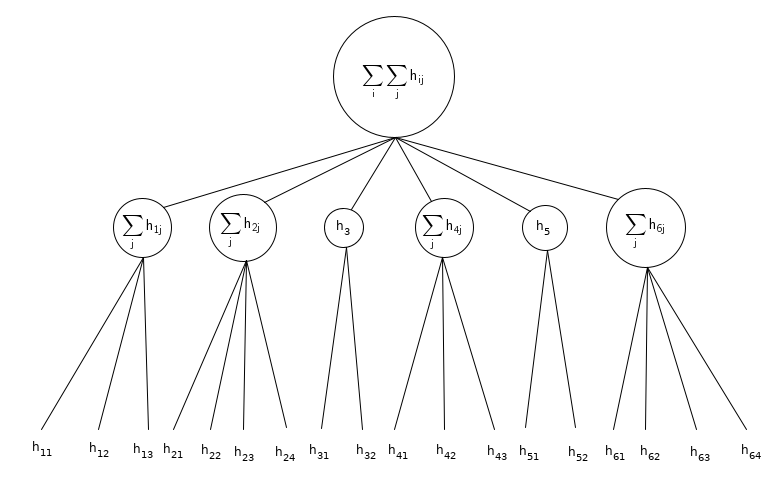
\includegraphics[width=0.8\linewidth]{Screenshot51}
	\caption{Иерархическая структура временных рядов, необходимых для анализа}
	\label{fig:screenshot51}
\end{figure}



\end{frame}

\begin{frame}[shrink=5]
\frametitle{Анализ предметной отрасли} 


	
	\begin{table} \small\centering\setlength{\extrarowheight}{0.25em}
		
		\begin{tabular}{   >{\centering\footnotesize}p{5.5em} 
				>{\centering\footnotesize}p{8em}
				>{\centering\footnotesize}p{5.5em} 
				>{\centering\footnotesize\arraybackslash}p{12em} }\hline
			
			
			
			Авторы, год & Название работы & Источник & Результат \\\hline 
			M. Cobb (2017) & Joint Forecast Combination of Macroeconomic Aggregates and Their Components  & MPRA Paper from University Library of Munich & Использование оптимальной комбинации прогнозов дает более точные прогнозы агрегированного ряда, по сравнению с суммой прогнозов каждого ряда по отдельности. \\
			R. Hyndman et al. (2010) & Optimal combination forecasts for hierarchical time series  & Computational Statistics \& Data Analysis & Корректировка прогнозов с помощью OLS  позоволяет сохранить иерархическую структуру рядов \\
			Justin L. Tobias (2001) & Forecasting output growth rates and median output growth rates: a hierarchical Bayesian approach  & Journal of Forecasting & Прогнозы можно улучшить за счет  стягивания оценок коэффициентов для нижних рядов к групповым оценкам.\\\hline
		\end{tabular}
	\end{table}


\end{frame}



\begin{frame}[shrink=3]
\frametitle{Цели и задачи} 


	\begin{block}{Актуальность:}
	\begin{itemize}
		
		\item  необходимость     прогнозирования иерархических рядов в микроэкономике,     макроэкономике, страховании, демографии.  
		%		\item  выявление факторов, позволяющих улучшить прогнозы агрегированного временного ряда. 
		
	\end{itemize}
\end{block}

	\begin{block}{Цель:}
	\begin{itemize}

		\item  сравнение моделей, учитывающих иерархическую структуру данных.
%		\item  выявление факторов, позволяющих улучшить прогнозы агрегированного временного ряда. 
		
	\end{itemize}
		
	\end{block}

	\begin{block}{Задачи:}
	\begin{itemize}

\item  сбор данных;
\item  выбор моделей;
\item  прогнозирование рядов второго и третьего уровня;
\item  сравнение суммы и оптимальной комбинации прогнозов.
%\item  сравнение прогнозов по рядам второго и третьего уровня. 


	\end{itemize}




	
\end{block}
\end{frame}



\begin{frame}[shrink=5]
\frametitle{Сбор данных с иерархической структурой} 

% Please add the following required packages to your document preamble:
% \usepackage{multirow}
		
\begin{table}[]
	
	\small\centering\setlength{\extrarowheight}{0.25em}
	
	\begin{tabular}{   >{\centering\footnotesize}p{8em} 
			>{\centering\footnotesize}p{4em} 
			>{\centering\footnotesize}p{4em} 
			>{\centering\footnotesize}p{4em} 
			>{\centering\footnotesize\arraybackslash}p{6em} }\hline

		
		
\multirow{2}{*}{\begin{tabular}[c]{@{}c@{}}Агрегированный\\ ряд\end{tabular}} & \multicolumn{3}{c}{Ряды второго уровня} & \multirow{2}{*}{\begin{tabular}[c]{@{}c@{}}Число рядов \\ третьего уровня\end{tabular}} \\
& по регионам & по типам & по кластерам &  \\\hline
ВВП ЕС & 28 & 10 & 25 & 280 \\
ВВП США & 50 & 21 & 25 & 1050 \\
ЕП РФ & 80 & 4 & 25 & 320\\\hline

	\end{tabular}
\end{table}


\begin{table}[]
	
	\small\centering\setlength{\extrarowheight}{0.25em}
	
	
	
	\begin{tabular}{   >{\centering\footnotesize}p{8em} 
			>{\centering\footnotesize}p{5em} 
			>{\centering\footnotesize}p{5em} 
			>{\centering\footnotesize}p{4em} 
			>{\centering\footnotesize\arraybackslash}p{4em} }\hline
		
		\multirow{2}{*}{\begin{tabular}[c]{@{}c@{}}Агрегированный\\ ряд\end{tabular}} & \multirow{2}{*}{Сезонность} & \multirow{2}{*}{\begin{tabular}[c]{@{}c@{}}Число\\ наблюдений\end{tabular}} & \multicolumn{2}{c}{Кросс-валидация} \\
		&  &  & \begin{tabular}[c]{@{}c@{}}число\\ подвыборок\end{tabular} & \begin{tabular}[c]{@{}c@{}}ширина\\ окна\end{tabular} \\\hline
		ВВП ЕС & 4 & 75 & 6 & 48 \\
		ВВП США & 4 & 54 & 6 & 28 \\
		ЕП РФ & 12 & 157 & 5 & 84\\\hline
	\end{tabular}
\end{table}



\end{frame}


\begin{frame}[shrink=5]
\frametitle{Сравнение суммы и оптимальной комбинации } 
\framesubtitle{Визуализация  месячных  временных рядов   }

\vfil
\hfil\hfil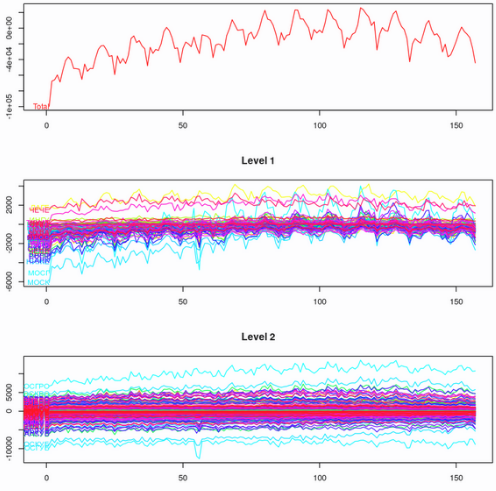
\includegraphics[height=6cm]{screenshot066}\hfil\hfil
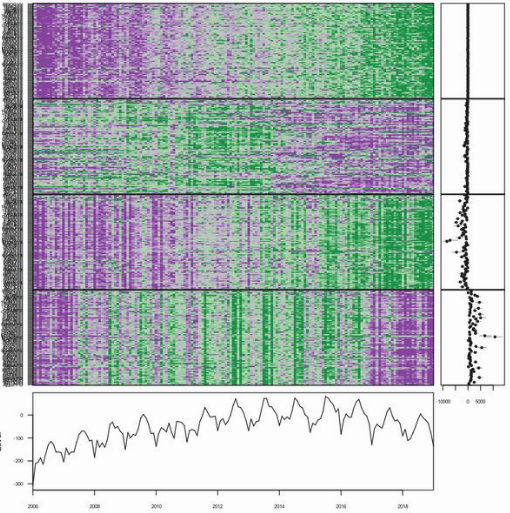
\includegraphics[height=6cm]{screenshot067}\newline
\null\hfil\hfil\makebox[5cm]{Три уровня агрегации}
\hfil\hfil\makebox[5cm]{Группировка по типам }
\end{frame}


% Please add the following required packages to your document preamble:
% \usepackage{multirow}




%
%\begin{frame}[shrink=5]
%\frametitle{\insertsection} 
%\framesubtitle{\insertsubsection}
%	\hfil\hfil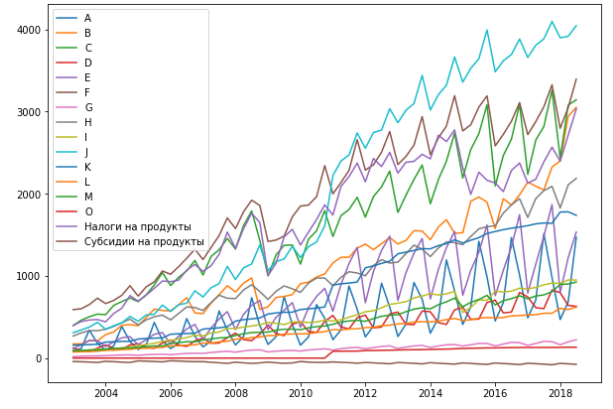
\includegraphics[width=5cm]{screenshot016}\newline
%	\null\hfil\hfil\makebox[5cm]{ВВП квартальный (производственный метод):}\newline
%	\vfil
%	\hfil\hfil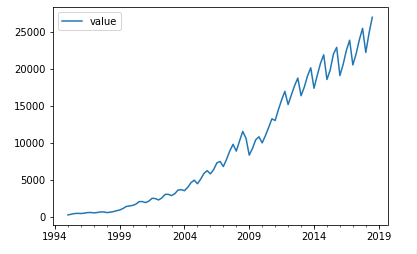
\includegraphics[width=5cm]{screenshot017}\hfil\hfil
%	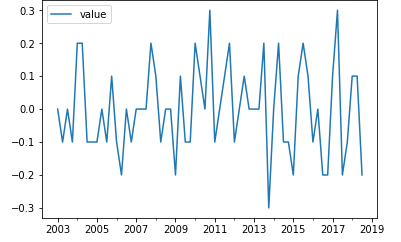
\includegraphics[width=5cm]{screenshot018}\newline
%	\null\hfil\hfil\makebox[5cm]{ВВП квартальный}
%	\hfil\hfil\makebox[5cm]{Разница (не более 0.00006 \%)}
%\end{frame}
%
%




\begin{frame}[shrink=5]
\frametitle{Выбор моделей} 
\begin{table}[]
\caption{Параметры моделей}
 \small\centering\setlength{\extrarowheight}{0.25em}	
	\begin{tabular}{   >{\centering\footnotesize}p{3em} 
			>{\centering\footnotesize}p{9.5em}
			>{\centering\footnotesize}p{3em} 
			>{\centering\footnotesize}p{4em} 
			>{\centering\footnotesize}p{4em} 			
			>{\centering\footnotesize}p{3em} 
			>{\centering\footnotesize\arraybackslash}p{4em} }\hline
		
		
		
		&                                                                                     & \multicolumn{2}{c}{ Квартальные} &  Сезонно \\ сглаженные & \multicolumn{2}{c}{ Месячные}    \\\hline
		&                                                                                     & $(p,d,q)$    & $(P,D,Q)_{4}$    & $(p,d,q)$          & $(p,d,q)$     & $(P,D,Q)_{12}$  \\\hline
		AR    &с линейным трендом,\\малым числом лагов& $(2,0,0)$    & $(1,0,0)$        & $(2,0,0)$  & $(2,0,0)$     & $(1,0,0)$       \\
		AR    & с линейным трендом                                                                  & $(3,0,0)$    & $(2,0,0)$        & $(4,0,0)$  & $(11,0,0)$    & $(2,0,0)$       \\
		AR    & с квадратичным трендом                                                              & $(3,0,0)$    & $(2,0,0)$        & $(4,0,0)$  & $(11,0,0)$    & $(2,0,0)$       \\
		AR    & интегированная                                                                      & $(3,1,0)$    & $(2,1,0)$        & $(4,1,0)$  & $(4,0,0)$     & $(1,1,0)$       \\
		ARMA  & с линейным трендом                                                                  & $(3,0,1)$    & $(2,0,1)$        & $(4,0,1)$  & $(4,0,1)$     & $(1,0,1)$       \\
		ARIMA &                                                                                     & $(3,1,1)$    & $(2,1,1)$        & $(4,1,1)$  & $(4,1,1)$     & $(1,1,1)$       \\\hline
		ETS   & $(E,T,S)=$                                                                          & \multicolumn{2}{c}{$(M,M,M)$}   & $(A,A,A)$          & \multicolumn{2}{c}{$(A,Ad,A) $} \\\hline
		TBATS & $trend =$                                                                           & \multicolumn{2}{c}{$A$}         & $A$                & \multicolumn{2}{c}{$Ad$} \\\hline       
	\end{tabular}

	\

$(p,d,q)$ -- параметры для ARIMA модели, $(P,D,Q)_{m}$ -- параметры для SARIMA модели с периодичностью $m$, $A$ - аддитивный, $Ad$ - аддитивный демпфированный, $M$ - мультипликативный. 


\end{table}


\end{frame}




\begin{frame}[shrink=5]
\frametitle{Сравнение суммы и оптимальной комбинации } 
\framesubtitle{Оптимальная комбинация прогнозов}

\begin{equation}\label{key123}
\begin{bmatrix}
y_{t} \\
y_{1, t} \\
y_{2, t} \\
... \\
y_{i, t} \\
y_{11, t} \\
y_{12, t} \\
y_{13, t} \\
y_{21, t} \\
y_{22, t} \\
y_{23, t} \\

... \\
y_{ij-2, t} \\
y_{ij-1, t} \\
y_{ij, t}
\end{bmatrix}
=
\begin{bmatrix}
1& 1 &1& 1& 1& 1& ... &1& 1& 1 \\
1 &1& 1& 0& 0& 0& ... &0 &0 &0  \\
0 &0 &0 &1& 1& 1& ... &0 &0 &0  \\
0& 0& 0& 0& 0& 0& ...&0 &0 &0 \\ 
0& 0& 0& 0& 0& 0& ...& 1& 1& 1 \\
1 &0 &0& 0& 0& 0& ...& 0& 0& 0 \\
0 &1 &0& 0& 0& 0& ...& 0& 0& 0 \\
0 &0 &1& 0& 0& 0& ...& 0& 0& 0 \\
0 &0 &0& 1& 0& 0& ...& 0& 0& 0 \\
0 &0 &0& 0& 1& 0& ...& 0& 0& 0 \\
0 &0 &0& 0& 0& 1& ...& 0& 0& 0 \\
0& 0& 0& 0& 0& 0& ...&0 &0 &0  \\ 
0 &0 &0& 0& 0& 0& ...& 1& 0& 0 \\
0 &0 &0& 0& 0& 0& ...& 0& 1& 0 \\
0 &0 &0& 0& 0& 0& ...& 0& 0& 1 
\end{bmatrix}
\begin{bmatrix}
y_{11, t} \\
y_{12, t} \\
y_{13, t} \\
y_{21, t} \\
y_{22, t} \\
y_{23, t} \\

... \\
y_{ij-2, t} \\
y_{ij-1, t} \\
y_{ij, t}
\end{bmatrix}
\end{equation}

\end{frame}


\begin{frame}[shrink=5]
\frametitle{Сравнение суммы и оптимальной комбинации } 
\framesubtitle{Оптимальная комбинация прогнозов}


\begin{equation}\label{key}
y_t  = S b_t ,
\end{equation}

\noindent
где $y_t$ -- вектор всех наблюдений на всех уровнях иерархии в момент времени $t$, $S$  -- суммирующая матрица
$ b_t $ -- вектор всех наблюдений на самом нижнем уровне иерархии в момент времени $t$



	\begin{block}{Невзвешенная сумма:}
\begin{equation}\label{key}
\tilde{y}_h = S \hat{y}_{K,h}   ,
\end{equation}
\end{block}
\begin{block}{OLS-корректировка:}
\begin{equation}\label{abc}
\hat{y}_h = S \beta_h + e_h  ,
\end{equation}
\begin{equation}\label{key555}
\tilde{y}_h
= S \hat{\beta}_h  = S ( S'  S )^{-1}  S'    \hat{y}_h .
\end{equation}
где $\tilde{y}_h$  -- собранные с помощью суммирования прогнозы рядов уровней $1...K-1$  и базовые прогнозы $\hat{y}_{K,h}$. 


\end{block}


\end{frame}









\begin{frame}[shrink=5]
\frametitle{Сравнение суммы и оптимальной комбинации } 
\framesubtitle{Процентное изменение RMSE для квартальных рядов}
	
	\vfil
	\hfil\hfil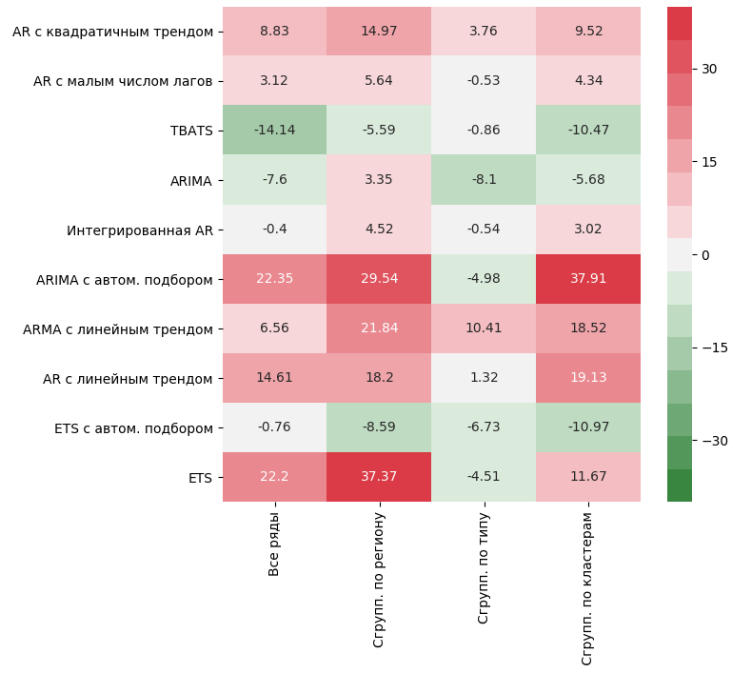
\includegraphics[height=6.5cm]{screenshot056}\hfil\hfil
	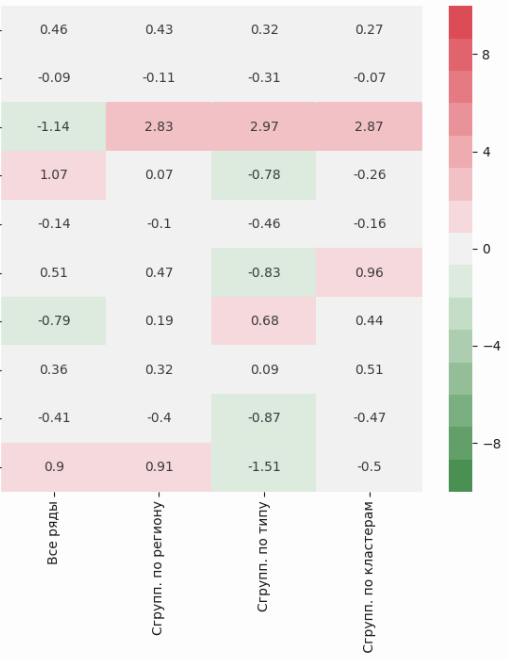
\includegraphics[height=6.5cm]{screenshot059}\newline
	\null\hfil\hfil\makebox[5cm]{Невзвешенная сумма}
	\hfil\hfil\makebox[5cm]{OLS-корректировка}
\end{frame}



\begin{frame}[shrink=5]
\frametitle{Сравнение суммы и оптимальной комбинации } 
\framesubtitle{Процентное изменение RMSE для квартальных сезонно-сглаженных  рядов}

\vfil
\hfil\hfil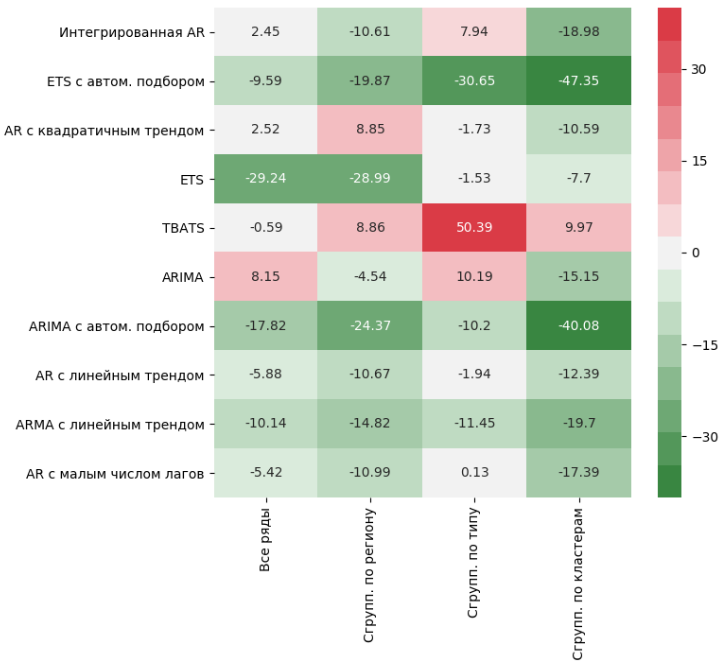
\includegraphics[height=6.5cm]{screenshot057}\hfil\hfil
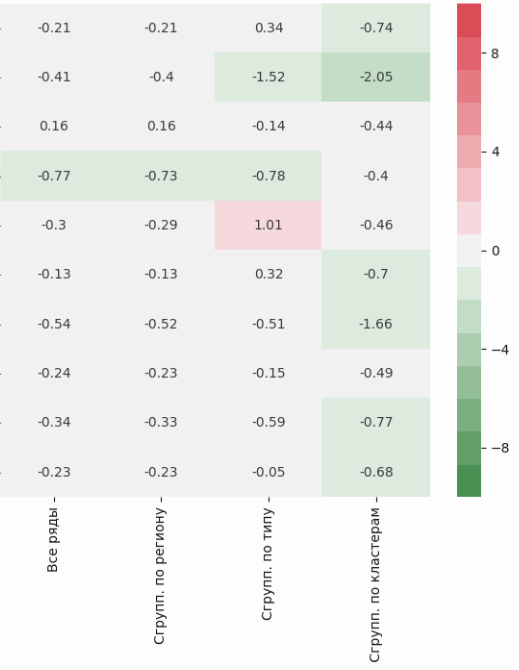
\includegraphics[height=6.5cm]{screenshot060}\newline
\null\hfil\hfil\makebox[5cm]{Невзвешенная сумма}
\hfil\hfil\makebox[5cm]{OLS-корректировка}
\end{frame}


\begin{frame}[shrink=5]
\frametitle{Сравнение суммы и оптимальной комбинации } 
\framesubtitle{Процентное изменение RMSE для месячных рядов}

\vfil
\hfil\hfil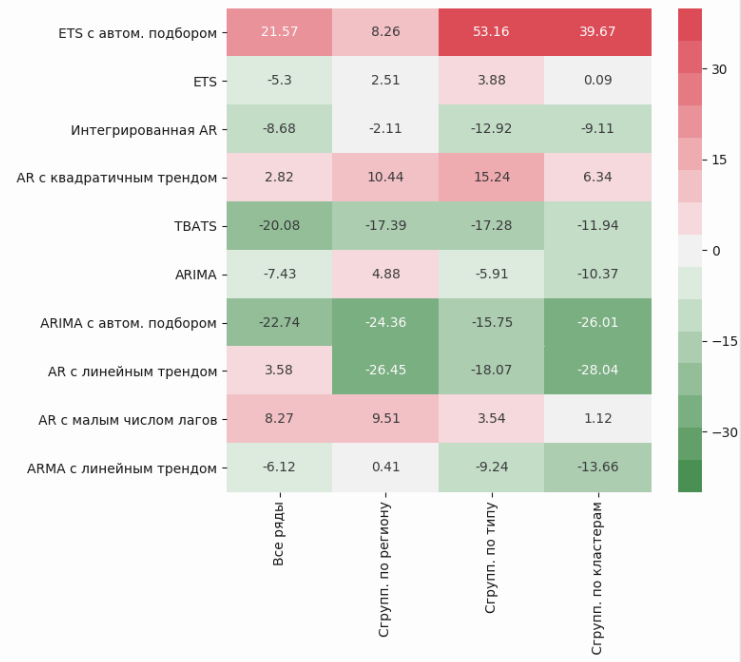
\includegraphics[height=6.5cm]{screenshot058}\hfil\hfil
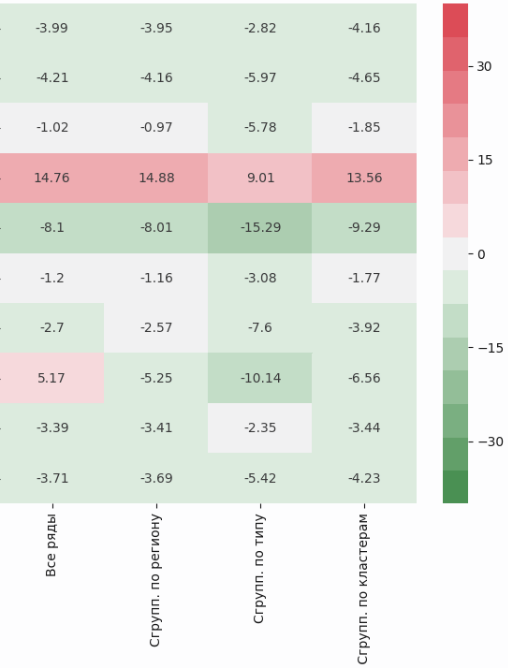
\includegraphics[height=6.5cm]{screenshot061}\newline
\null\hfil\hfil\makebox[5cm]{Невзвешенная сумма}
\hfil\hfil\makebox[5cm]{OLS-корректировка}
\end{frame}






\begin{frame}[shrink=3]
\frametitle{Результат исследования} 


\begin{block}{Результат:}

\

	\begin{itemize}


\item  эффективность прогнозирования сильно варьируется в зависимости от характеристик наборов данных и их  рядов-компонент;

\

\item  корректировка прогнозов с помощью OLS позволяет избавиться от случайного накопления идиосинкразических ошибок;

\

\item  группировка рядов  улучшает прогнозы  по сравнению с прогнозами полученными по трехуровневой модели. 		


	\end{itemize}
	
\end{block}




\end{frame}








\begin{frame}[c, plain]
\begin{center}
	
	\bigskip
	
	
	{\LARGE Спасибо за внимание!}
	
	\bigskip
	
	{\Large \inserttitle}
	
	\bigskip
	
	{\insertauthor} 
	
	\bigskip
	
	\bigskip\bigskip
	
	{\large \insertdate}
\end{center}
\end{frame}







\begin{frame}[shrink=3]

\frametitle{Актуальность и основные гипотезы} 




\begin{block}{Актуальность:}
	\begin{itemize}
		
		\item  точный прогноз экономических показателей – один из ключевых факторов принятия эффективных решений;
		
		\item  необходимость прогнозирования данных с иерархической структурой в микроэкономике, макроэкономике, страховании, демографии;
		
		\item  применение иерархических моделей на трех наборах данных с использованием кросс-валидации позволит получить более устойчивые выводы.
		
	\end{itemize}
	
\end{block}

\begin{block}{Гипотезы:}
	\begin{itemize}
		\item  при группировке рядов, которые ведут себя одинаково, идиосинкразичесие ошибки внутри групп будут компенсировать друг друга, в то время общая динамика будет сохраняться;
		
		\item  подбор весов с помощью регрессии позволяет учесть более точные прогнозы с большим весом. 
	\end{itemize}
	
\end{block}
\end{frame}


\begin{frame}[shrink=5]
\frametitle{Сравнение суммы и оптимальной комбинации } 
\framesubtitle{Визуализация  квартальных временных рядов   }

\vfil
\hfil\hfil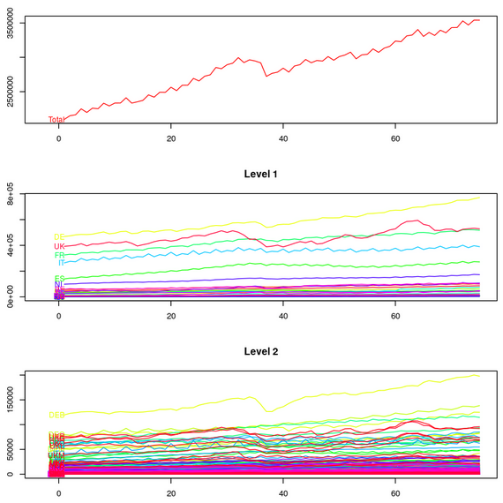
\includegraphics[height=6cm]{screenshot062}\hfil\hfil
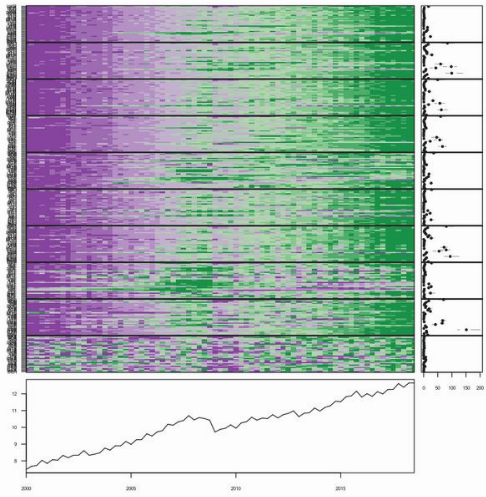
\includegraphics[height=6cm]{screenshot063}\newline
\null\hfil\hfil\makebox[5cm]{Три уровня агрегации}
\hfil\hfil\makebox[5cm]{Группировка по отраслям }
\end{frame}


\begin{frame}[shrink=5]
\frametitle{Сравнение суммы и оптимальной комбинации } 
\framesubtitle{Визуализация  квартальных сезонно-сглаженных временных рядов   }

\vfil
\hfil\hfil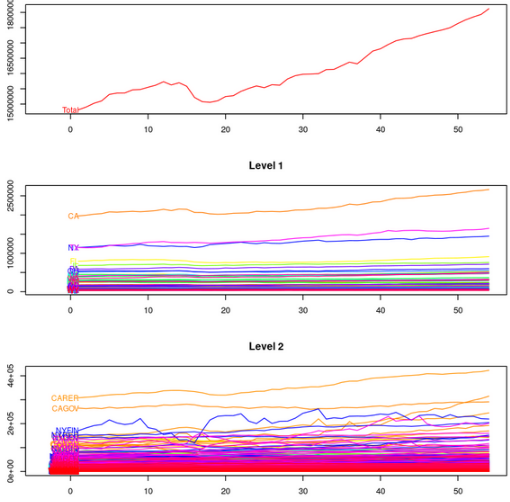
\includegraphics[height=6cm]{screenshot064}\hfil\hfil
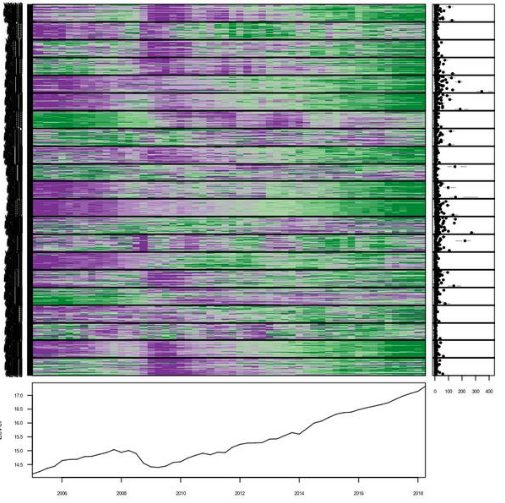
\includegraphics[height=6cm]{screenshot065}\newline
\null\hfil\hfil\makebox[5cm]{Три уровня агрегации}
\hfil\hfil\makebox[5cm]{Группировка по отраслям }
\end{frame}


\begin{frame}[shrink=5]
\frametitle{Сравнение прогнозов} 
\framesubtitle{Временные ряды сгруппированные по евклидовой метрике}

\vfil
\hfil\hfil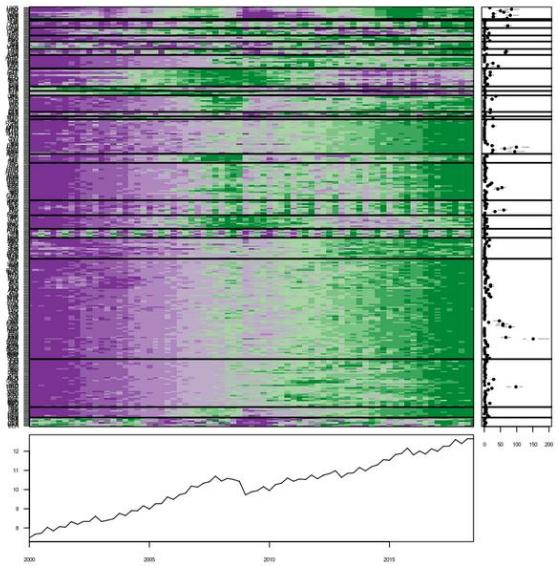
\includegraphics[height=4cm]{screenshot068}\hfil\hfil
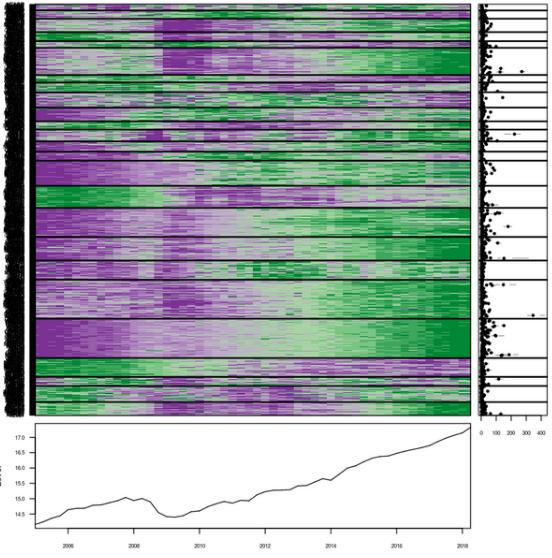
\includegraphics[height=4cm]{screenshot069}\hfil\hfil
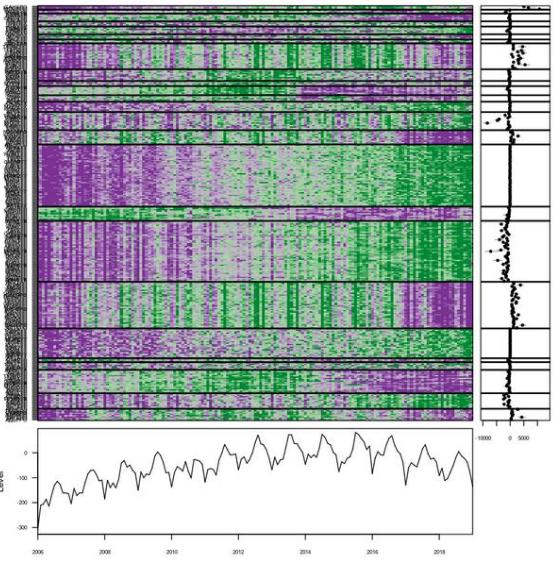
\includegraphics[height=4cm]{screenshot070}
\newline
\null\hfil\hfil\makebox[4cm]{ВВП ЕС}
\hfil\hfil\makebox[4cm]{ВВП США}
\hfil\hfil\makebox[4cm]{ЕП РФ}
\end{frame}


\begin{frame}[shrink=5]
\frametitle{Сравнение суммы и оптимальной комбинации } 


Квадратный корень из среднеквадратичной ошибки (root mean square error):
\begin{equation}\label{key}
RMSE = \sqrt{  \frac{1}{h} \sum_{i=1}^h(\hat{y}_{t+i|t}-y_{t+i})^2}
\end{equation}


Евклидова метрика:
\begin{equation}\label{key}
d(y_{i,t},y_{j,t}) = \sqrt{\sum^T_{t=1} (y_{i,t} - y_{j,t}  )^2 }, 
\end{equation}

Индекс силуэта для кластерной структуры: 
\begin{equation}\label{key}
SI = \frac{1}{N} \sum^N_{i=1} S_{y_i}=\frac{1}{N} \sum^N_{i=1} \dfrac{b_{pi}-a_{pi}}{\max(a_{pi}, b_{pi})},
\end{equation}

\end{frame}





\end{document}